\begin{frame}{Industria Cloro-Álcali}
  \frametitle{Un Uso Residual en Proceso de Extinción}
  Históricamente, el mayor uso industrial del mercurio fue en la producción de cloro y sosa cáustica.

  \begin{itemize}[<+->]
    \item En este proceso, el mercurio actúa como cátodo líquido para producir una amalgama de sodio ($Na-Hg$) de alta pureza.
    \item \textbf{Estado actual:} Esta tecnología se considera obsoleta. La mayoría de los países han forzado la conversión a tecnologías más seguras, como las celdas de membrana.
    \item Quedan muy pocas plantas operativas y están bajo una estricta regulación para su cierre definitivo.
  \end{itemize}
\end{frame}

\begin{frame}{Iluminación Especializada}
  \frametitle{Aplicaciones de Nicho en Lámparas de Descarga}
  Cantidades muy pequeñas de mercurio son todavía esenciales para ciertos tipos de lámparas.

  \begin{columns}[T]
    \begin{column}{0.6\textwidth}
      \begin{itemize}[<+->]
        \item El vapor de mercurio genera luz UV que excita el fósforo en \textbf{lámparas fluorescentes (CFL)} y tubos lineales.
        \item También se usa en lámparas de descarga de alta intensidad (HID) y en \textbf{lámparas UV germicidas}.
        \item \textbf{Sustitución:} La tecnología \textbf{LED} está reemplazando rápidamente a las lámparas fluorescentes debido a su mayor eficiencia y ausencia de mercurio.
      \end{itemize}
    \end{column}
    \begin{column}{0.4\textwidth}
      \begin{figure}
        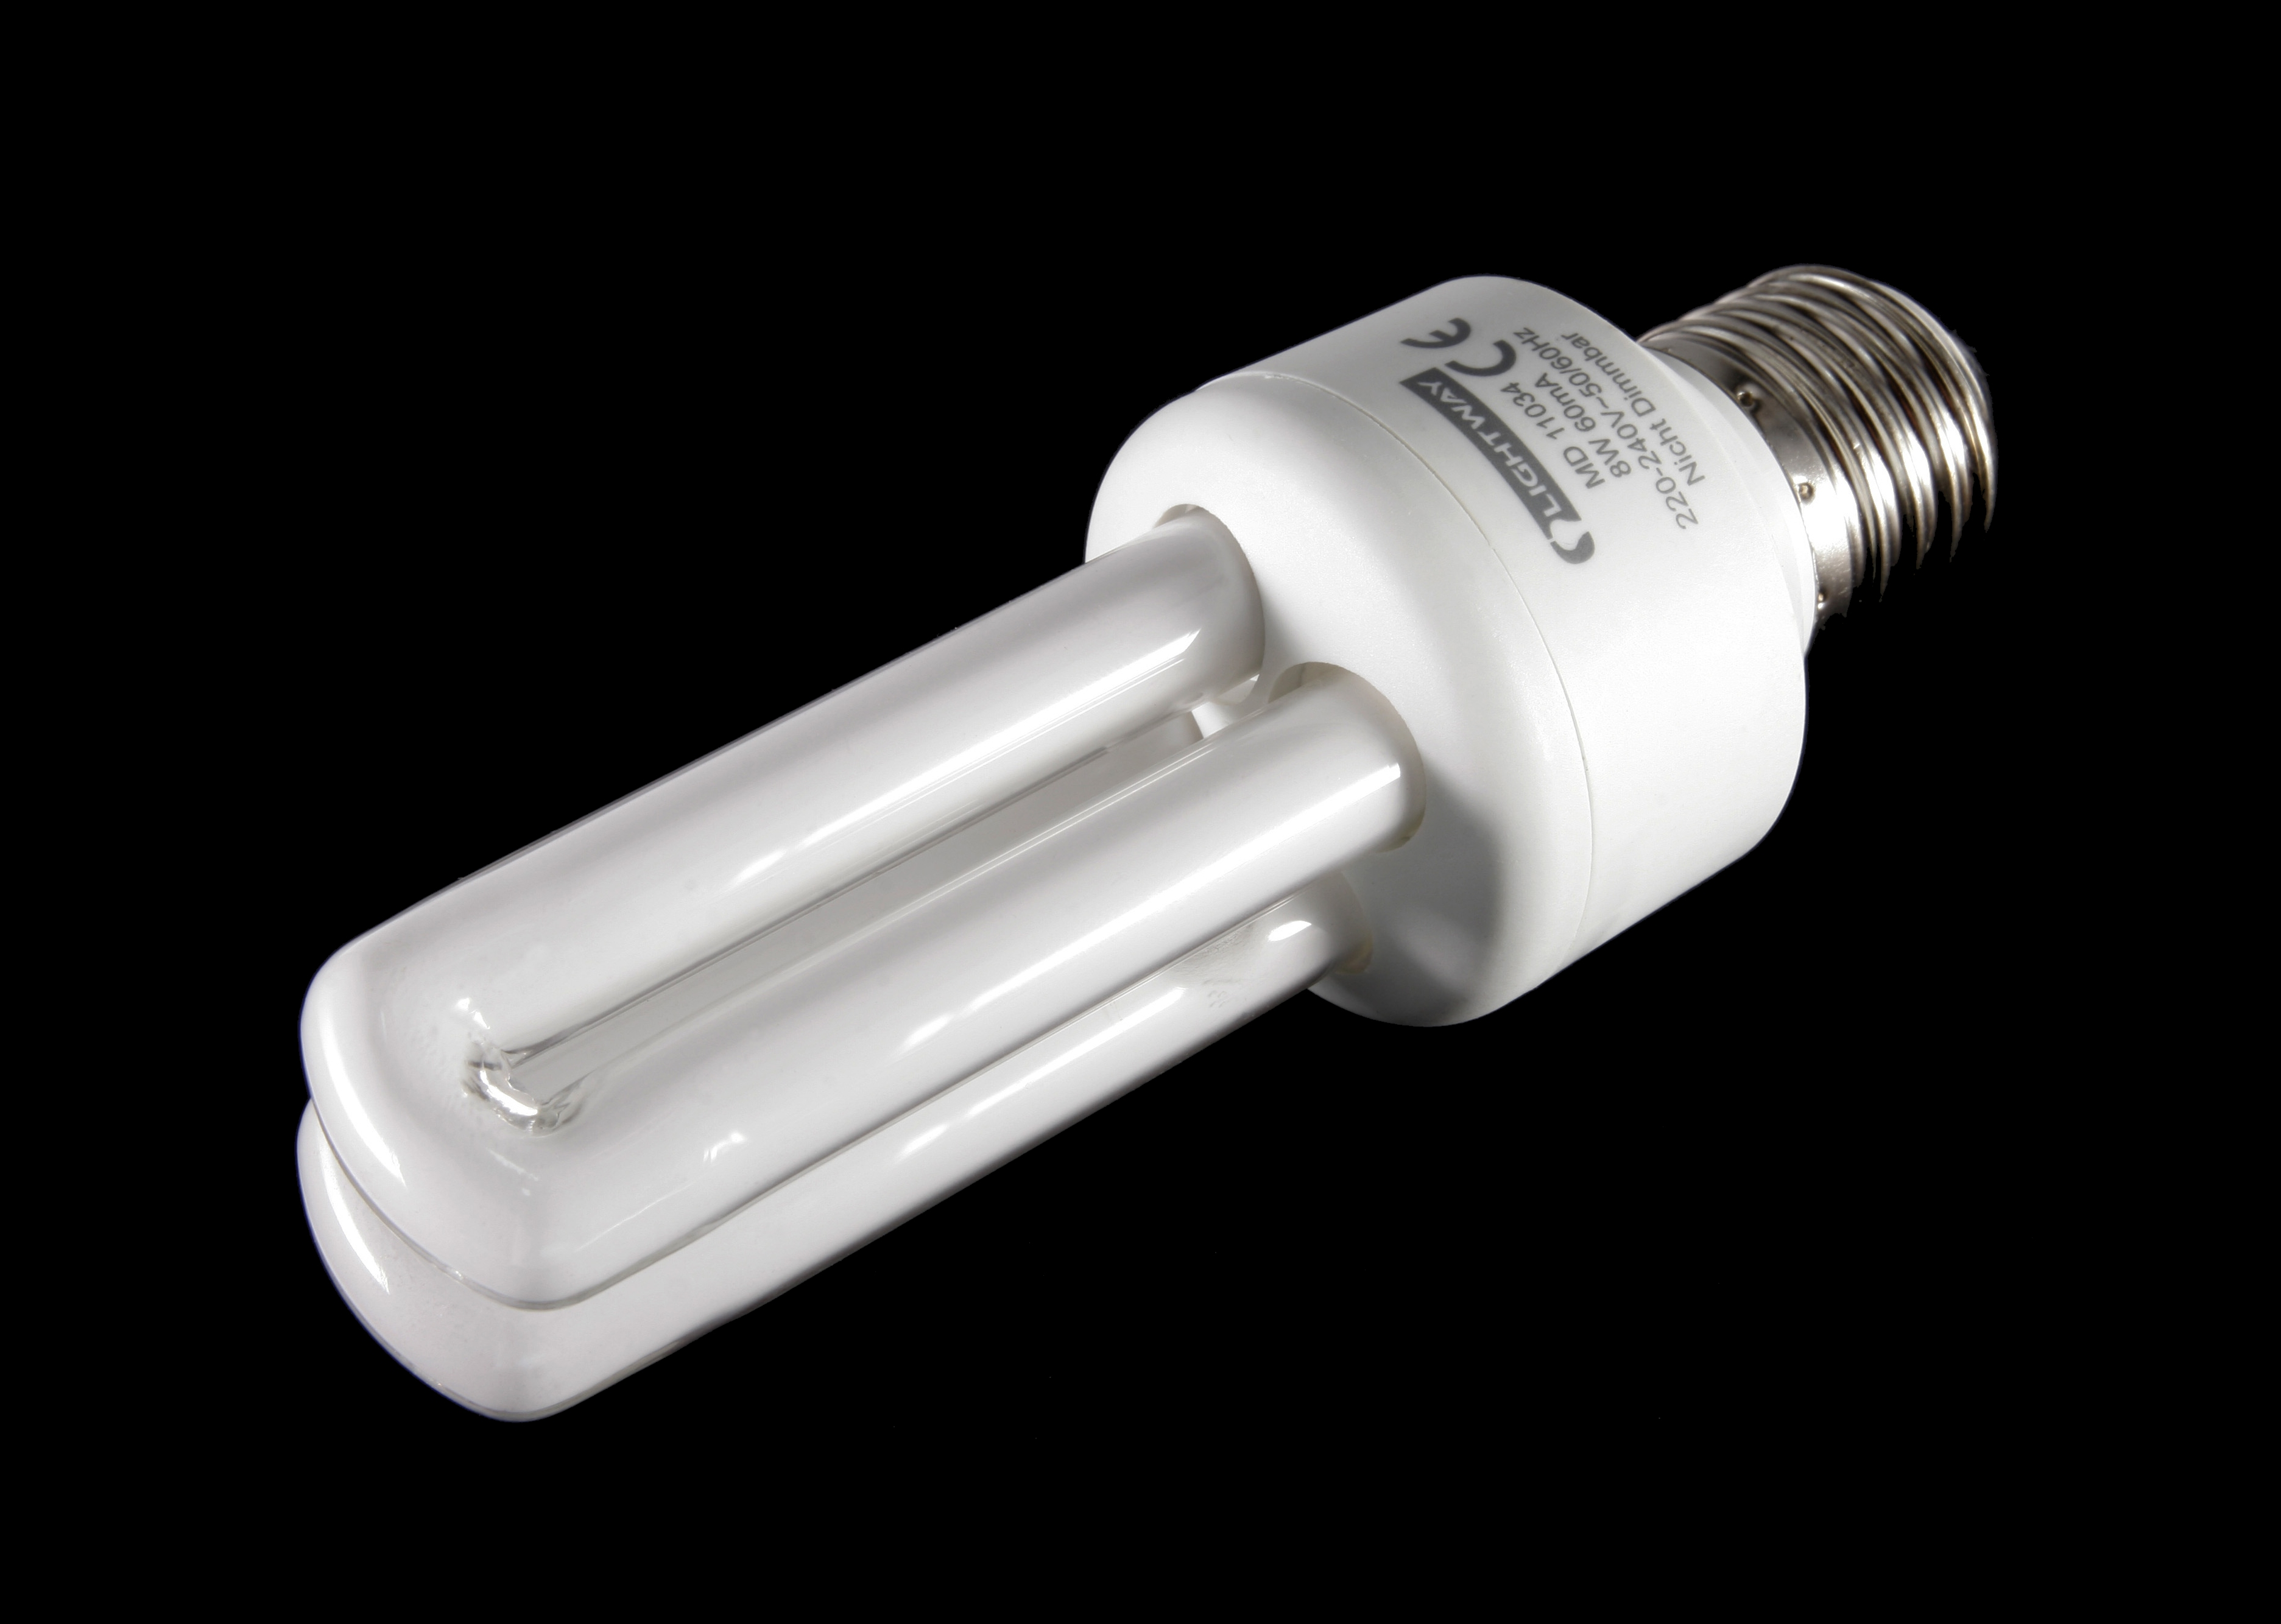
\includegraphics[width=\textwidth]{../figures/cfl_lamp.jpg} % Reemplaza con la ruta a tu imagen
        \caption{Lámpara Fluorescente Compacta (CFL). \tiny{Fuente: Wikipedia}}
      \end{figure}
    \end{column}
  \end{columns}
\end{frame}

\begin{frame}{Instrumentación Científica y de Control}
  \frametitle{Usos Altamente Especializados y de Referencia}
  Las propiedades del mercurio lo mantienen como un material de referencia en aplicaciones científicas críticas.

  \begin{columns}[T]
    \begin{column}{0.6\textwidth}
      \begin{itemize}[<+->]
        \item \textbf{Porosimetría de mercurio:} Es una técnica estándar para medir la porosidad en materiales. No existe un sustituto directo con la misma precisión.
        \item \textbf{Electrodos de referencia:} Electrodos como el de calomelanos saturados ($Hg_2Cl_2$) son patrones en electroquímica por su potencial estable.
        \item \textbf{Sustitución:} Se prioriza el uso de termómetros y manómetros digitales en todas las aplicaciones no críticas.
      \end{itemize}
    \end{column}
    \begin{column}{0.4\textwidth}
      \begin{figure}
        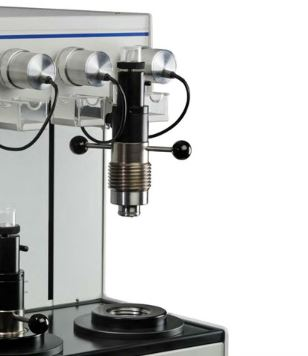
\includegraphics[width=\textwidth]{../figures/mercury_porosimeter.jpg} % Reemplaza con la ruta a tu imagen
        \caption{Equipo de porosimetría de mercurio. \tiny{Fuente: ATA Scientific Instruments}}
      \end{figure}
    \end{column}
  \end{columns}
\end{frame}

\begin{frame}{El Futuro: Una Industria Libre de Mercurio}
  \frametitle{Principales Vías de Innovación Tecnológica}
  La investigación se centra en eliminar los últimos bastiones del uso del mercurio.

  \begin{itemize}[<+->]
    \item \textbf{Catálisis:} Desarrollo de catalizadores libres de mercurio (ej. a base de oro) para la producción de cloruro de vinilo (PVC).
    \item \textbf{Amalgamas dentales:} Mejora de la durabilidad de resinas compuestas y los ionómeros de vidrio para reemplazarlas por completo.
    \item \textbf{Componentes electrónicos:} Desarrollo de interruptores de estado sólido (MEMS) para sustituir a los de mercurio en equipos especializados.
  \end{itemize}
\end{frame}

\begin{frame}{Puntos Importantes}
  \frametitle{Puntos importantes}
  \begin{itemize}[<+->]
    \item El rol del mercurio en la industria moderna se ha reducido drásticamente a unas pocas \textbf{aplicaciones de nicho}.
    \item El principal motor de la innovación es desarrollar \textbf{tecnologías de sustitución} eficientes (Convenio de Minamata).
    \item El futuro industrial del mercurio reside en la gestión segura de sus residuos y en la \textbf{remediación} de la contaminación histórica.
  \end{itemize}
\end{frame}